% Part (a): which matrices abliteration edits. Sized for ONE column.
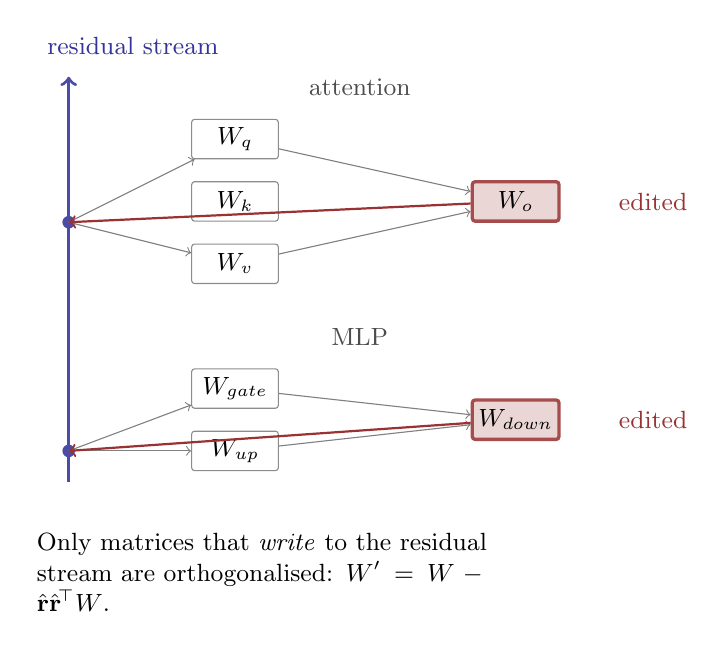
\begin{tikzpicture}[
  font=\small, x=1.32mm, y=1.32mm,
  blk/.style={draw=black!45, rounded corners=1pt, minimum width=11mm,
              minimum height=5mm, inner sep=1pt, fill=white, font=\small},
  edited/.style={blk, fill=Maroon!16, draw=Maroon!70, very thick},
  res/.style={draw=NavyBlue!70, very thick},
  lab/.style={font=\small, text=black!70},
]
\draw[res, ->] (0,7) -- (0,46);
\node[text=NavyBlue!80, font=\small, anchor=west] at (-3,49) {residual stream};
\foreach \y in {10,32} \fill[NavyBlue!70] (0,\y) circle (0.8mm);

% attention
\node[blk]    (q) at (16,40) {$W_q$};
\node[blk]    (k) at (16,34) {$W_k$};
\node[blk]    (v) at (16,28) {$W_v$};
\node[edited] (o) at (43,34) {$W_o$};
\draw[->, black!50] (0,32) -- (q); \draw[->, black!50] (0,32) -- (v);
\draw[->, black!50] (q) -- (o);    \draw[->, black!50] (v) -- (o);
\draw[->, Maroon!80, thick] (o) -- (0,32);
\node[lab] at (28,45) {attention};

% MLP
\node[blk]    (g) at (16,16) {$W_{\text{gate}}$};
\node[blk]    (u) at (16,10) {$W_{\text{up}}$};
\node[edited] (d) at (43,13) {$W_{\text{down}}$};
\draw[->, black!50] (0,10) -- (g); \draw[->, black!50] (0,10) -- (u);
\draw[->, black!50] (g) -- (d);    \draw[->, black!50] (u) -- (d);
\draw[->, Maroon!80, thick] (d) -- (0,10);
\node[lab] at (28,21) {MLP};

\node[lab, anchor=west, text=Maroon!80] at (52,34) {edited};
\node[lab, anchor=west, text=Maroon!80] at (52,13) {edited};
\node[anchor=north west, font=\small, text width=62mm] at (-4,3)
  {Only matrices that \emph{write} to the residual stream are orthogonalised:
   $W' = W - \hat{\mathbf r}\hat{\mathbf r}^{\!\top}W$.};
\end{tikzpicture}
